\begin{solution}
	 Seja $ z = x + y\,i $.
	 Fazendo $ x = 3 + 2 \cos{t} $ e $ y = -1 + 3 \sen{t} $, temos
	 \begin{align}
	  \cos{t} &= \frac{x - 3}{2} \label{cos}\\
	  \sen{t} &= \frac{y + 1}{3} \label{sen}
	 \end{align}
	 Elevado ao quadrado as equações \eqref{cos} e \eqref{sen}, e somando 
		membro a membro, encontramos:
	 \[
			\left( \frac{x - 3}{2} \right)^2 + \left (\frac{y + 1}{3} \right)^2 =
			\cos^{2}{t} + \sen^{2}{t}
			\Longrightarrow
			\Ovalbox{$\displaystyle\frac{(x-3)^2}{2^2}+\frac{(y-(-1))^2}{3^2}=1$}
		\]
  Ou seja, uma \emph{Elipse} de centro $ (3, -1) $ e de semieixos $ a = 2 $
		e $b=3$.
	 Veja a Figura~\ref{fig:elipse}.
  
  \begin{minipage}{\textwidth}
	  \centering
	  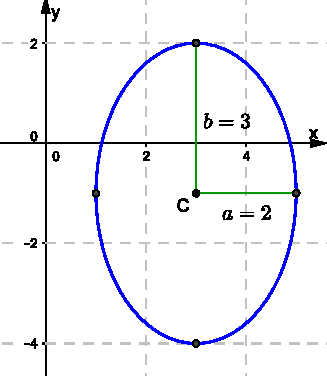
\includegraphics[width=5cm]{elipse}
	  \captionof{figure}{Conjunto dos complexos $z(t)$ visto geometricamente.}
	  \label{fig:elipse}
	 \end{minipage}  
\end{solution}